%# -*- coding:utf-8 -*-
\section{Experiments and Results}
\label{sec4_2}

\subsection{Medical Data and Experimental Setup}

The original chest CTA series was acquired by a 128-slice Siemens SOMATOM Definition Flash CT.
The slice thickness was $0.6 \text{mm}$ and the in-slice resolution was $0.4 \times 0.4 \text{mm}^2$.
Since the work was all on the coronary arteries, the volume contained the whole heart (i.e., ROI, which is the abbreviation of \textit{region of interest}) was cropped from the original data as shown in Fig. \ref{fig:Original}. %

Numbers of experiments were conducted with different sets of parameters to segment the coronary arteries from CTA for the testament of the approach in this paper.
In our case, the original CTA series in DICOM format had been converted to the form of XML first; and the data type of pixels are converted for the incoming computation.
Next the converted data was enhanced by the module which was implemented based on the algorithm developed in \cite{Sato1998}.
Then the tubular enhanced data was send to the following modules to perform calculations of speed image production and input level sets generation.
The two set of the resulting data from the two computation pipelines were transferred to the CURVES module in order to generate the final fronts evolution results.
Finally, the marching cubes method was employed to extract the iso-surface corresponding to the wall of the coronary arteries.
All the experiments were performed on a machine with Intel's 2.83GHz Core 2 Quad CPU and 4GB RAM.

\subsection{Tubular Enhancement and Its Postprocessing}

Before the tubular enhancement started, a global binary thresholding was performed in order to provide the enhancing filter with the focus on the tiny bright tubular objects.
To achieve this, the thresholder was called to trim the irrelevant contents in the images, e.g., dark lung regions with negative intensity values, bright bone regions with large positive intensity values, etc. %
As shown in Fig. \ref{fig:Binary1}, the intensity values of the regions within the interval between the lower threshold and the upper threshold were uniformly assigned a unique intensity value, i.e., $255$ in our case; the intensity values of the rest regions were uniformly assign a zero intensity value. %

Referring to the shape prior guidelines listed in Table. \ref{tbl:Eigenvalues}, the tubular enhancement filter was fed the parameters to detect the bright tubular objects, i.e., coronary arteries. %
Among these parameters, $\sigma$ controls the diameter of cross-section of the tubular objects to be enhanced, $\gamma_{12}$ is the measure of the tube similarity, and $\gamma_{23}$ is used for the recovery of vessel regions with inhomogeneous contrast or intensity loss. %
As shown in Fig. \ref{fig:Vesselness}, the tiny vessels including the coronary arteries and the vessels in lung areas were enhanced with a small $\sigma$ whilst the tubular structures with cross-section diameters larger than this value were not enhanced. %

The intensity values of the enhanced tubular objects were relatively low and scattered in a wide range.
This is a mass for the selection of the intensity value in the following processing steps.
To deal with it and facilitate this situation, some intensity transformation step was needed.
The nonlinear intensity mapping filter and the binary threshold filter were the candidates.

Equation (\ref{eqn:Sigmoid}) showed that the nonlinear intensity mapping transformed the input image into the image with partial enhancement and partial attenuation.
With the well chosen parameters, the intensity values corresponding to the targeting objects in this case were enlarged and the rest part of the images in lower intensities were all depressed as near zero intensity areas. %
Because of the mapping characteristics of the sigmoid functions, the intensity values of the bright tubular structures were not uniformly distributed and stayed at the relatively low levels (see Fig. \ref{fig:Sigmoid}). %
In another test, the binary threshold filter extracted the pixels with the intensities in the specified range and assigned them with a unique large intensity value as discussed above (see Fig. \ref{fig:Binary2}). %
Comparing the result of the two candidates, the binary threshold filter was selected to improve the results of the precedent tubular enhancement filter (see Fig. \ref{fig:DataFlow}). %
\begin{figure}[t]
\centering
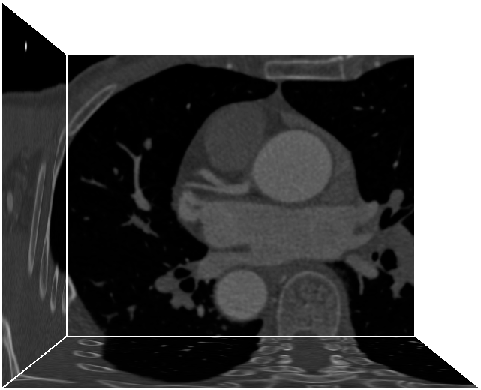
\includegraphics[width=2.8in]{Figures/chap04/original.png}
\caption{Original ROI-extracted volumetric data}
\label{fig:Original}
\end{figure}
\begin{figure}[t]
\centering
\subfloat[]{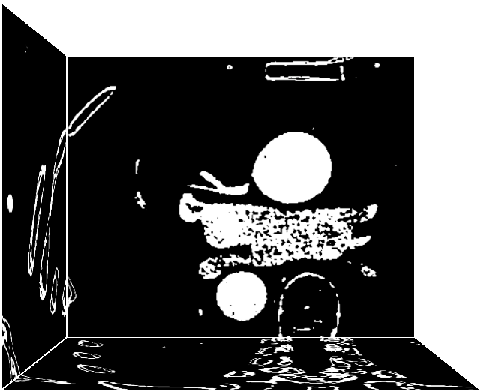
\includegraphics[width=2.8in]{Figures/chap04/binary1.png}%
\label{fig:Binary1}}
\hfil
\subfloat[]{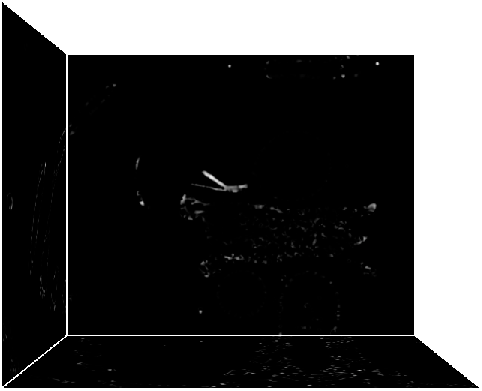
\includegraphics[width=2.8in]{Figures/chap04/hessian.png}%
\label{fig:Vesselness}}
\caption{Preprocessing results of the original CTA images based on the ``vesselness" measure: (a) binary thresholding ($\text{lower threshold} = 300$, $\text{upper threshold} = 600$) (b) tubular enhancement ($\sigma = 0.9$, $\gamma_{12} = 0.1$, $\gamma_{23} = 2.0$).}%
\label{fig:Preprocessing}
\end{figure}

\subsection{Feature Images Computation}

To generate the feature images for the CURVES system, two steps were performed:
(1) calculating the gradient magnitude at each pixel; and
(2) converting the gradient images into the speed images.
%\begin{enumerate}
%\item calculating the gradient magnitude at each pixel;
%\item converting the gradient images into the speed images.
%\end{enumerate}
The gradient magnitude module computed the magnitude of the gradient pixel-wisely for the image by performing the convolution with the first order derivatives of a Gaussian kernel.
The wall of the tiny vessels were extracted before the nonlinear intensity mapping was employed to generate the edge potential maps.
The extreme values of the pixel intensities in the gradient magnitude images directly effected the selection of the parameters in (\ref{eqn:Sigmoid}).
To reverse the lightness of the objects (in low intensities in the gradient magnitude images) and its edges (in high intensities in the gradient magnitude images), $n$ was chosen to be the center of the intensity window containing the vessels, and $m$ a negative value with $|m|$ as the width of the window. %
The minus sign of $m$ means the reverse operation on the pixels.
The neighborhood of the boundaries of the objects were in almost zero intensity, which made the evolution driven by (\ref{eqn:Application}) faster in the ``plateau" (with uniformly high intensities), whilst much slower (in a speed of about zero) in the ``ridges" (with rapid decreasing intensities). %

\subsection{Wave Fronts Propagation}

The initial level sets were evolved by the colliding fronts module.
Two seeds were located interior of the regions corresponding to the coronary arteries and the interfaces surrounding each seeds evolved towards each other.
The dot production of the gradients of arrival times of the two wavefronts were computed.
\begin{figure}[t]
\centering
\subfloat[]{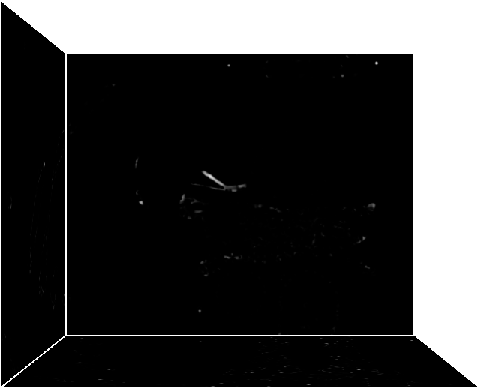
\includegraphics[width=2.8in]{Figures/chap04/sigmoid.png}%
\label{fig:Sigmoid}}
\hfil
\subfloat[]{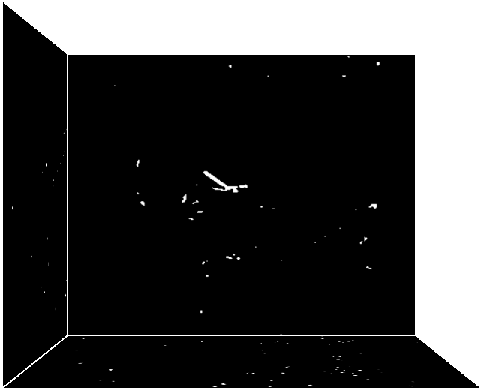
\includegraphics[width=2.8in]{Figures/chap04/binary2.png}%
\label{fig:Binary2}}
\caption{Comparison of the two different intensity conditioning approaches: (a) nonlinear intensity mapping ($m = 80$, $n = 120$); (b) binary thresholding ($\text{lower threshold} = 40$, $\text{upper threshold} = 200$).}%
\label{fig:IntensityConditioning}
\end{figure}
\begin{figure}[t]
\centering
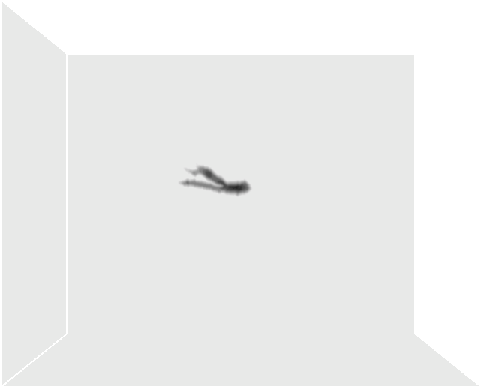
\includegraphics[width=2.8in]{Figures/chap04/curves.png}
\caption{CURVES evolution based on the initial contours generated by the colliding fronts method and the edge feature maps calculated by the nonlinear intensity mapping function.}%
\label{fig:CURVES}
\end{figure}
\begin{figure*}[t]
\centering
\subfloat[]{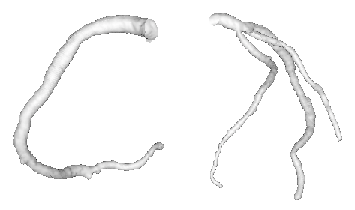
\includegraphics[width=2.8in]{Figures/chap04/model_conventional.png}%
\label{fig:VisualizationModelCURVES}}
\hfil
\subfloat[]{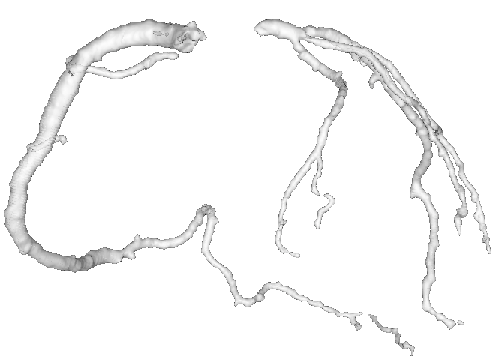
\includegraphics[width=2.4in]{Figures/chap04/model_enhanced.png}%
\label{fig:VisualizationModelTECURVES}}
\caption{Models of the coronary arteries: (a) conventional CURVES evolution; (b) tubular-enhanced CURVES evolution.}%
\label{fig:VisualizationModel}
\end{figure*}

The CURVES system started working when all the preceding calculation completed.
The module took the speed images as its evolution maps and the initial contours as its initial states and regulates the evolution according to (\ref{eqn:Application}).
The evolution terminated when the contours evolved against the wall of the coronary arteries in the specified steps of iterations.
And the resulting evolution extracted the coronary arteries as shown in Fig. \ref{fig:CURVES}.
Next a binary thresholding step was provoked to label the inner area of the coronary arteries with high intensity value whilst the outer area with zero intensity value.

\subsection{Visualization of Segmentation Results}

By manually picked the isovalue corresponding to the wall of the coronary arteries, the resulting volume were processed using the marching cubes method \cite{Lorensen1987MC}.
The visualization models of the coronary arteries respectively based on the CURVES regions without and with tubular enhancement demonstrated their capabilities of displaying the complicated geometrical details (see Fig. \ref{fig:VisualizationModelCURVES} and \ref{fig:VisualizationModelTECURVES}). %
